\section{Results}
\label{sec:results}

\subsection{Claim 1}

\todo{TRISTAN}

\subsection{Claim 2}

Our reproduction of Claim~2 was ultimately unsuccessful.
While the paper reports a clear output-logit divergence when weight decay is
removed, we did not observe the same phenomenon reliably in our small-scale
setting.
Across the runs we carried out, the mean output logit either remained
comparatively well-behaved, or training became unstable in a more global and
less interpretable way before any clean divergence pattern emerged.

To make the instability easier to trigger, we deliberately explored more
aggressive training settings than our default setup.
In particular, we disabled gradient clipping, increased the learning rate,
removed learning-rate warmup, and disabled learning-rate decay.
These changes were intended to stress the optimisation dynamics and reproduce
the failure mode described in the paper more quickly.
However, this did not lead to a convincing confirmation of the claim.

Instead, we observed two broad outcomes.
In some runs, training remained stable enough that the output logit mean did
not exhibit the expected runaway behaviour, even in the no-weight-decay
configuration.
In other runs, optimisation became unstable more abruptly, with large training
pathologies that made the behaviour difficult to attribute specifically to the
output-logit mechanism discussed by~\citet{wortsman2023smallscale}.
As a result, our experiments do not provide clear evidence that removing weight
decay alone causes the output logit mean to explode in our setting, nor do they
allow us to cleanly isolate the stabilising effect of z-loss.

We nevertheless report representative figures from these runs.
They illustrate the main outcome of our reproduction attempt: depending on the
configuration, we observed either no clear divergence in the output logit mean
or severe overall optimisation instability, but not the clean qualitative
pattern described in the original paper.

\begin{figure}[t]
    \centering

    % -------- Row 1: Stable --------
    \begin{subfigure}{0.48\textwidth}
        \centering
        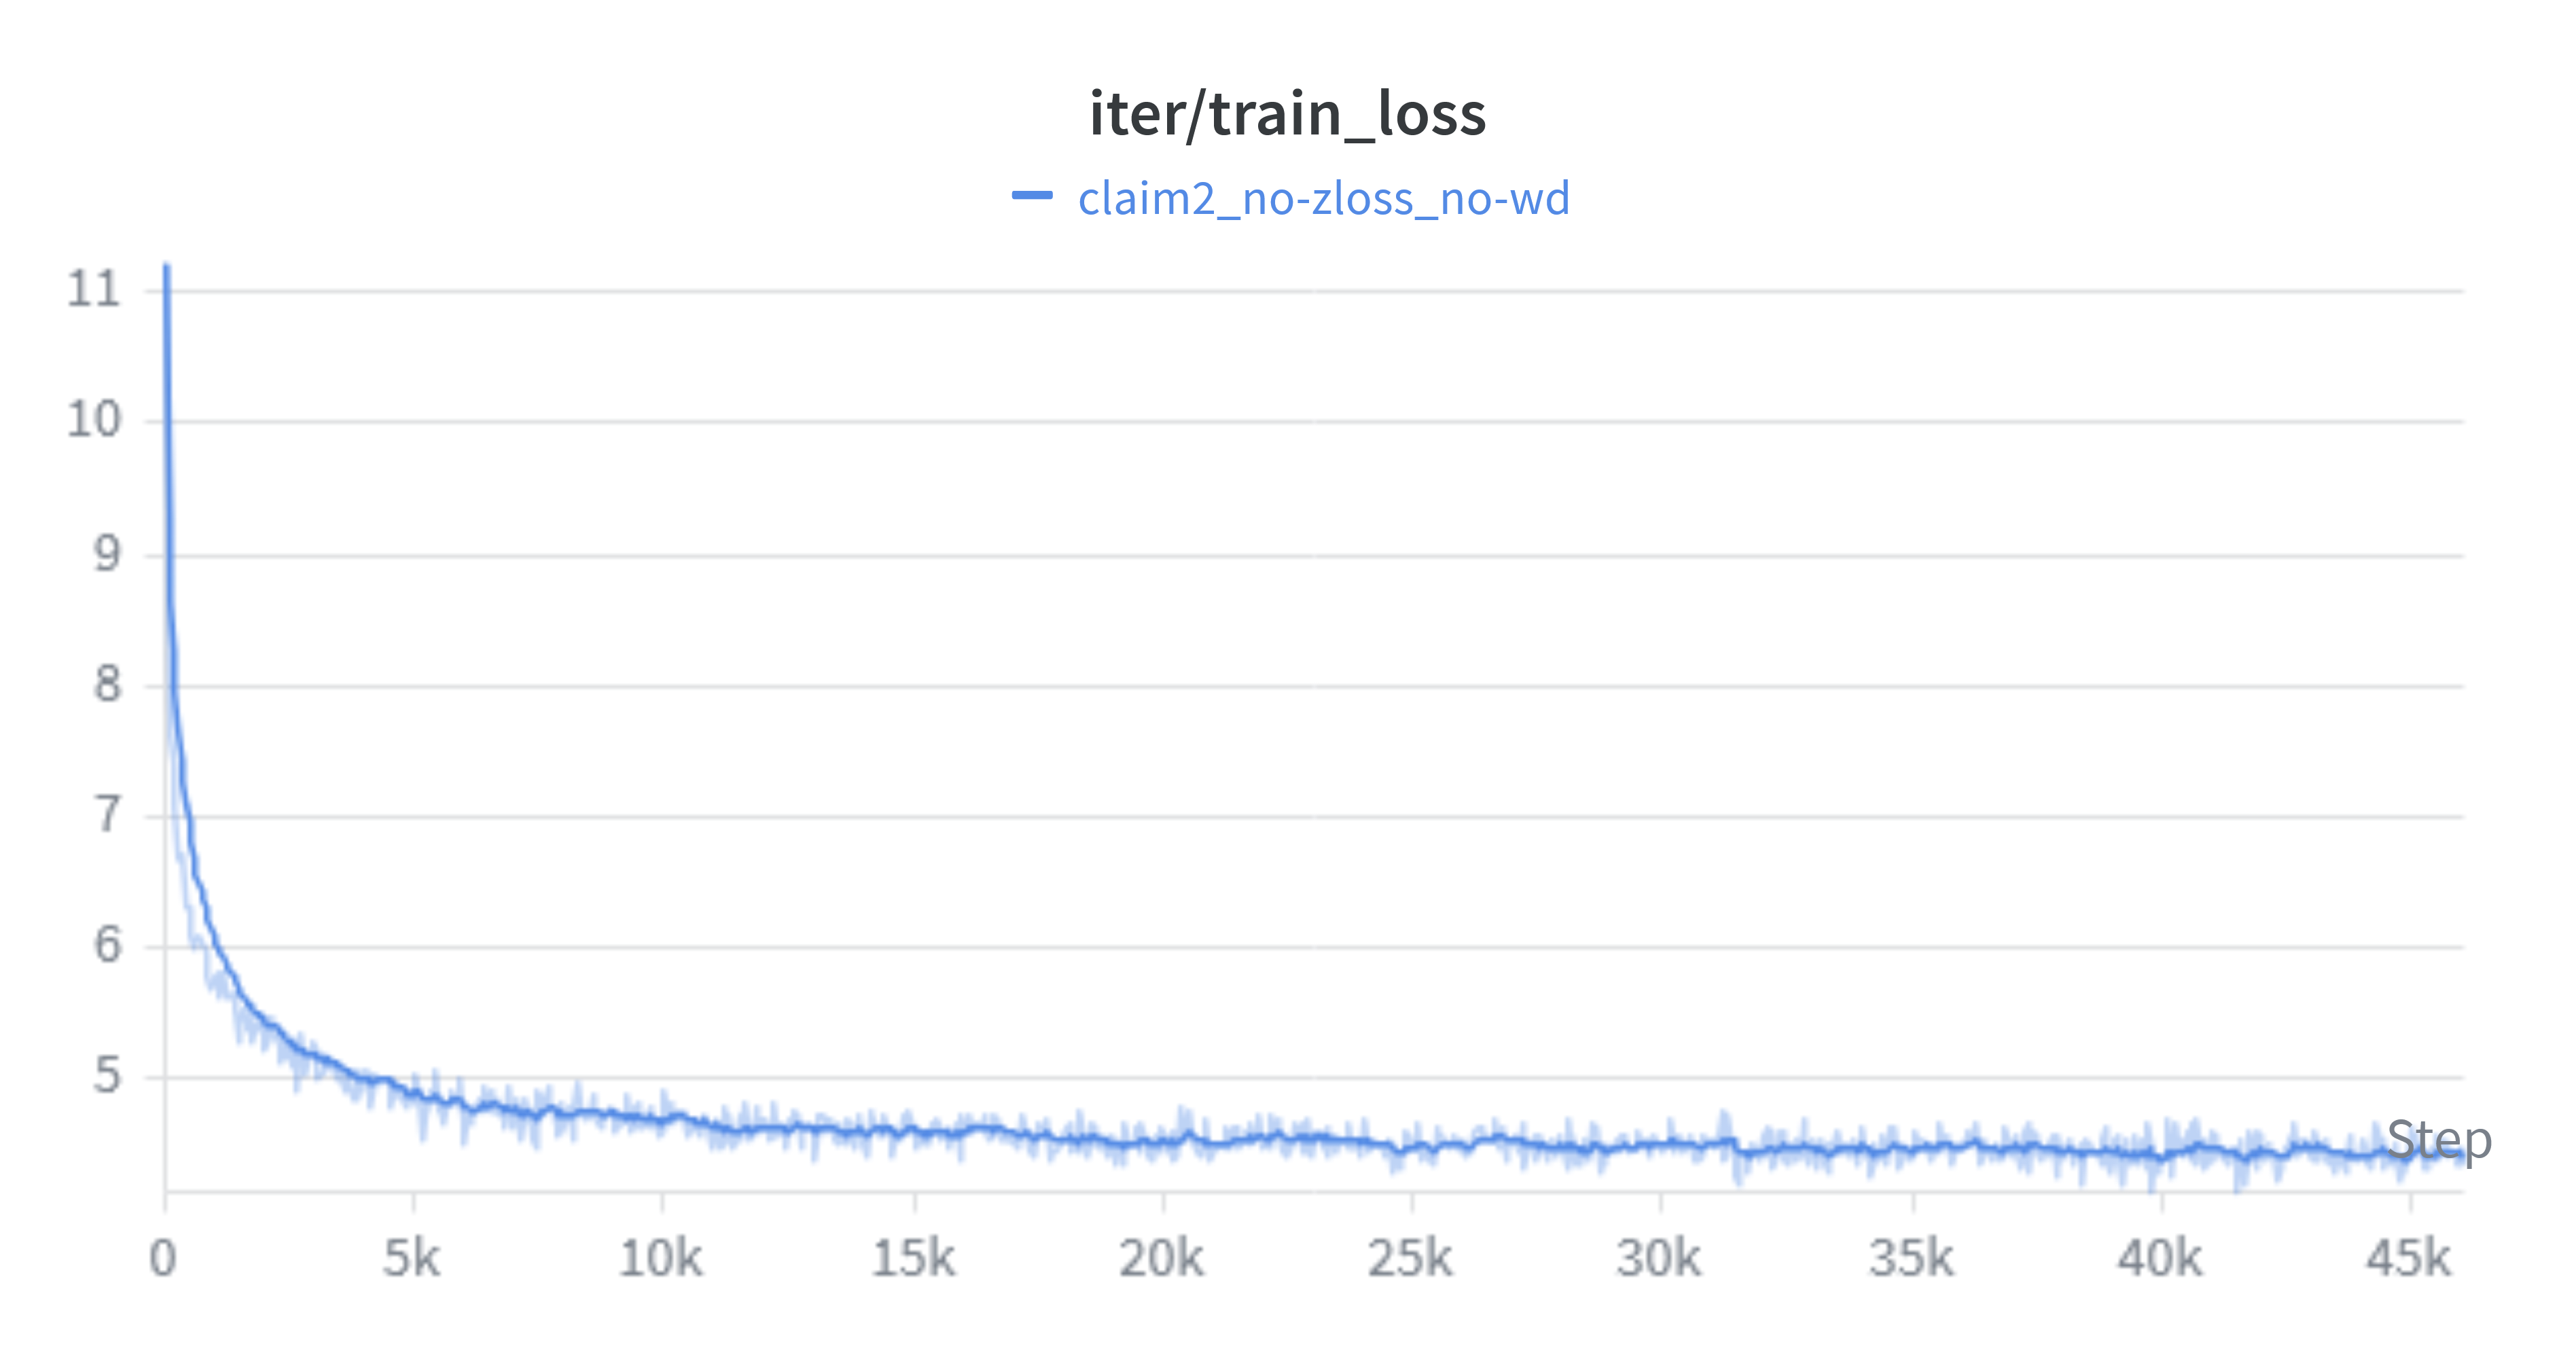
\includegraphics[width=\linewidth]{figures/C2_train_loss_stable.png}
        \caption{Stable — train loss}
    \end{subfigure}
    \hfill
    \begin{subfigure}{0.48\textwidth}
        \centering
        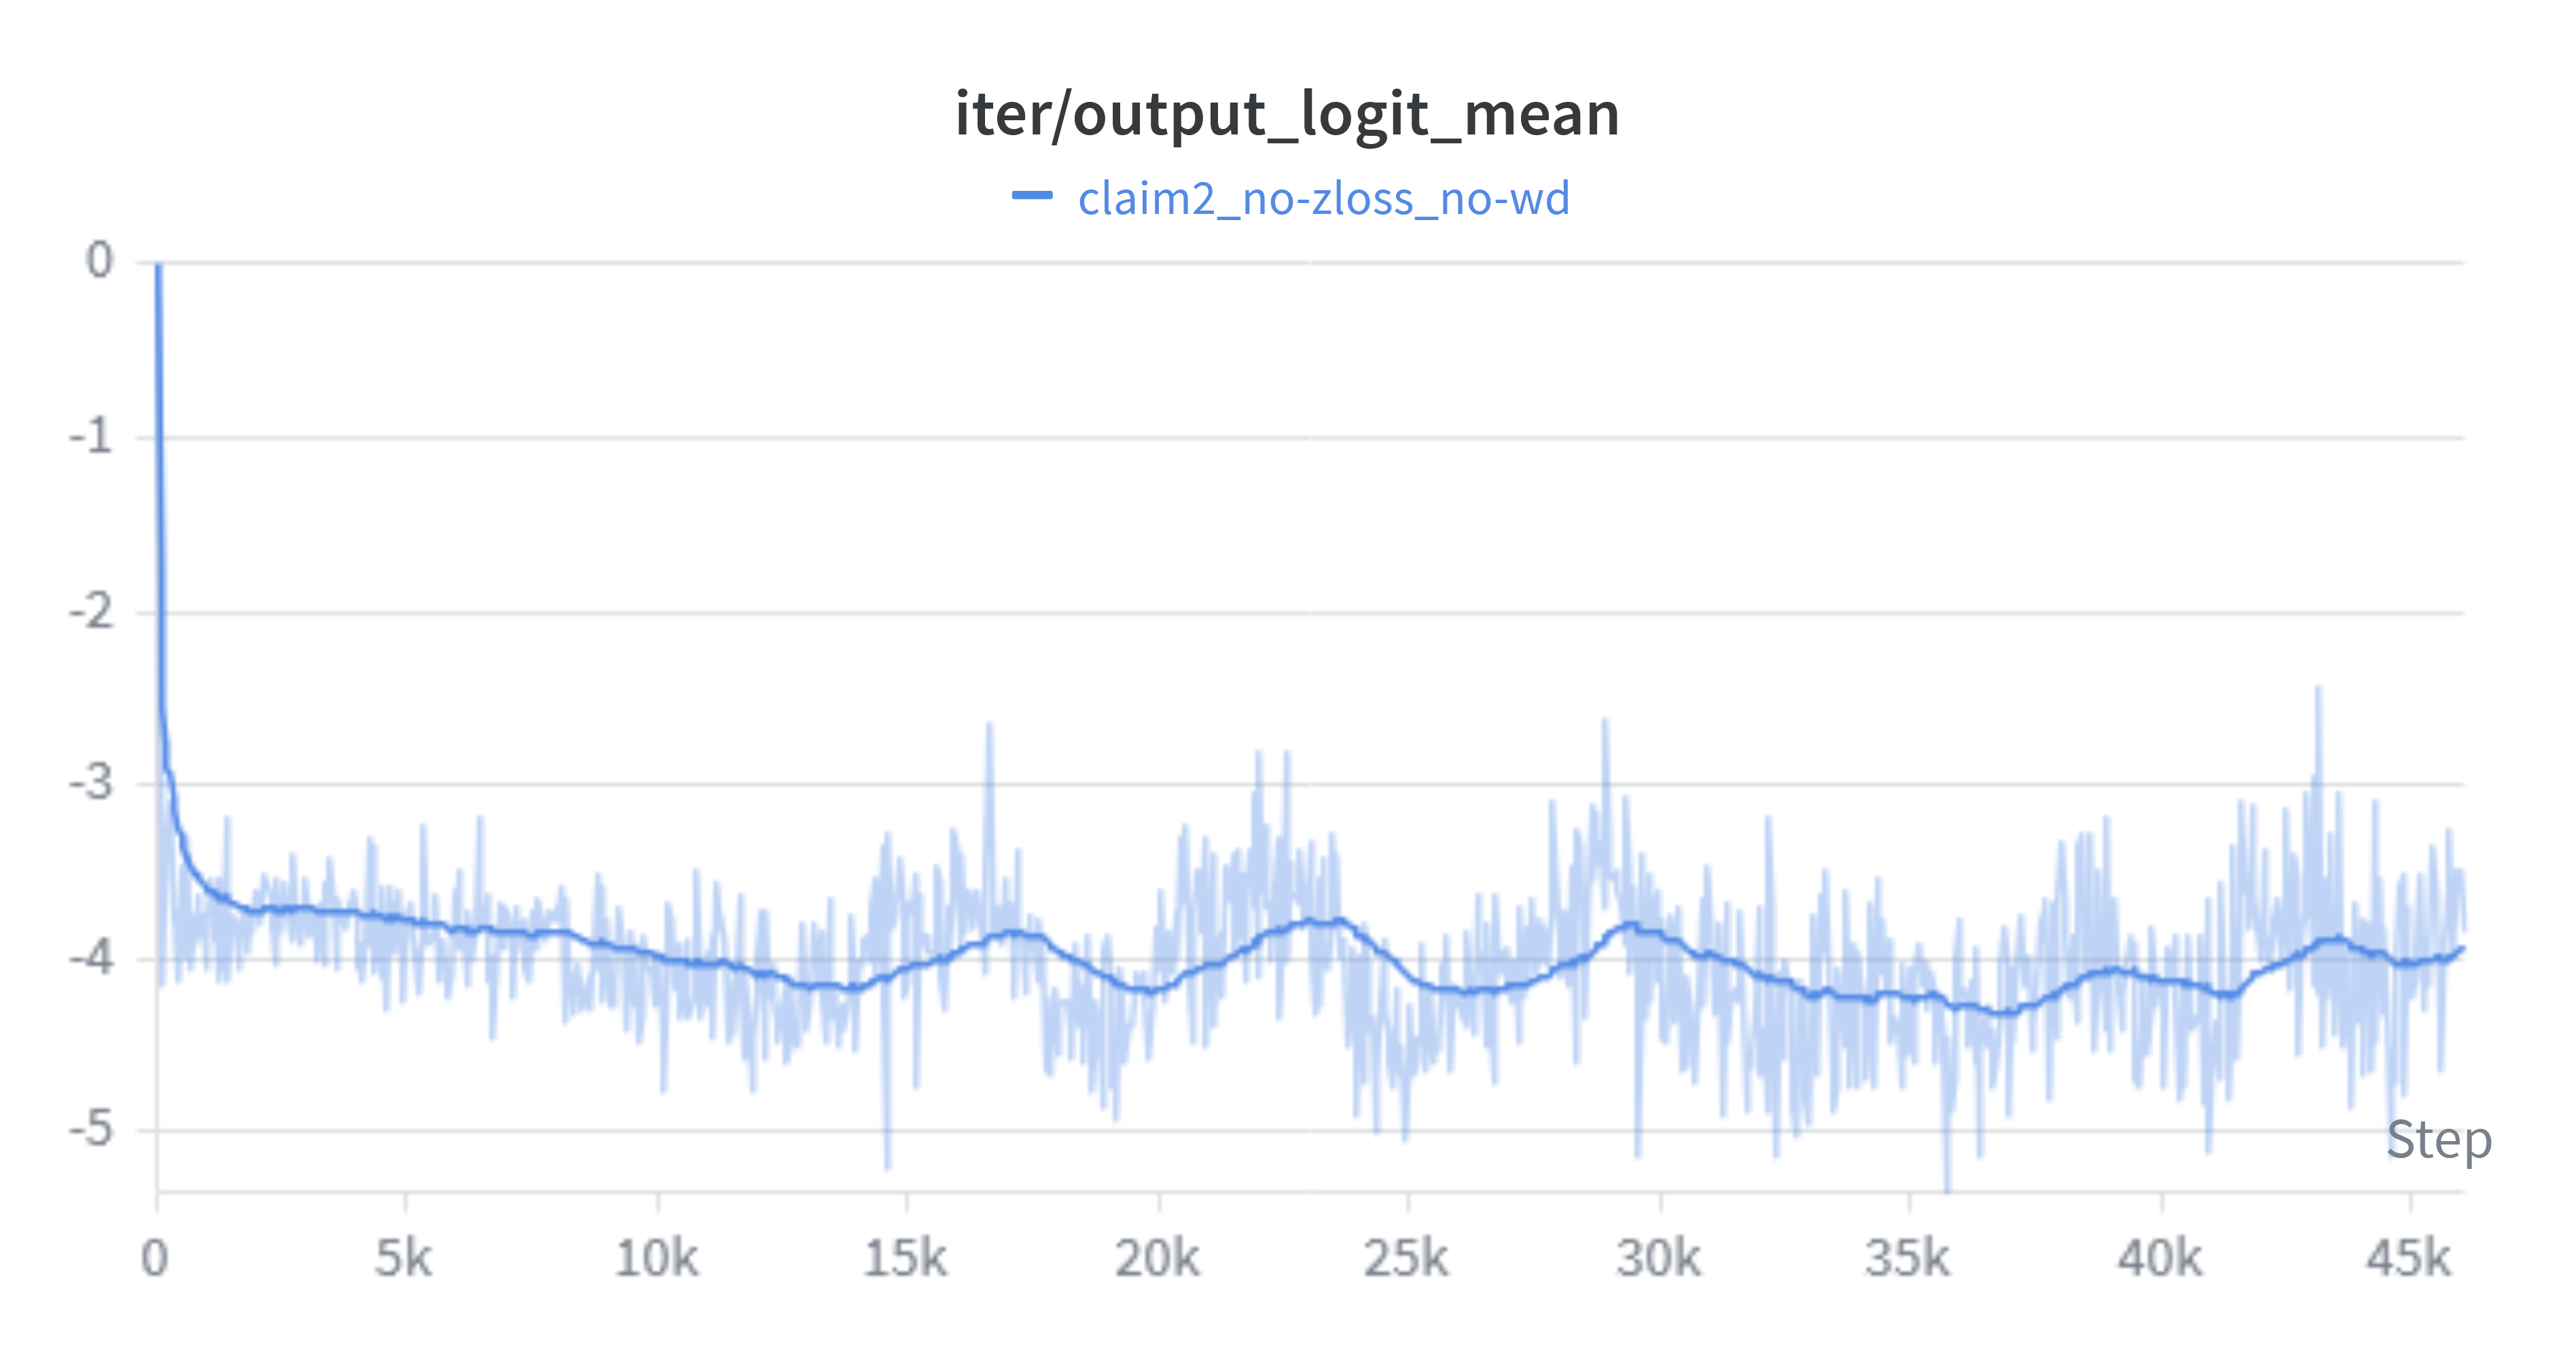
\includegraphics[width=\linewidth]{figures/C2_logit_mean_stable.png}
        \caption{Stable — logit mean}
    \end{subfigure}

    \vspace{0.5em}

    % -------- Row 2: OK stable --------
    \begin{subfigure}{0.48\textwidth}
        \centering
        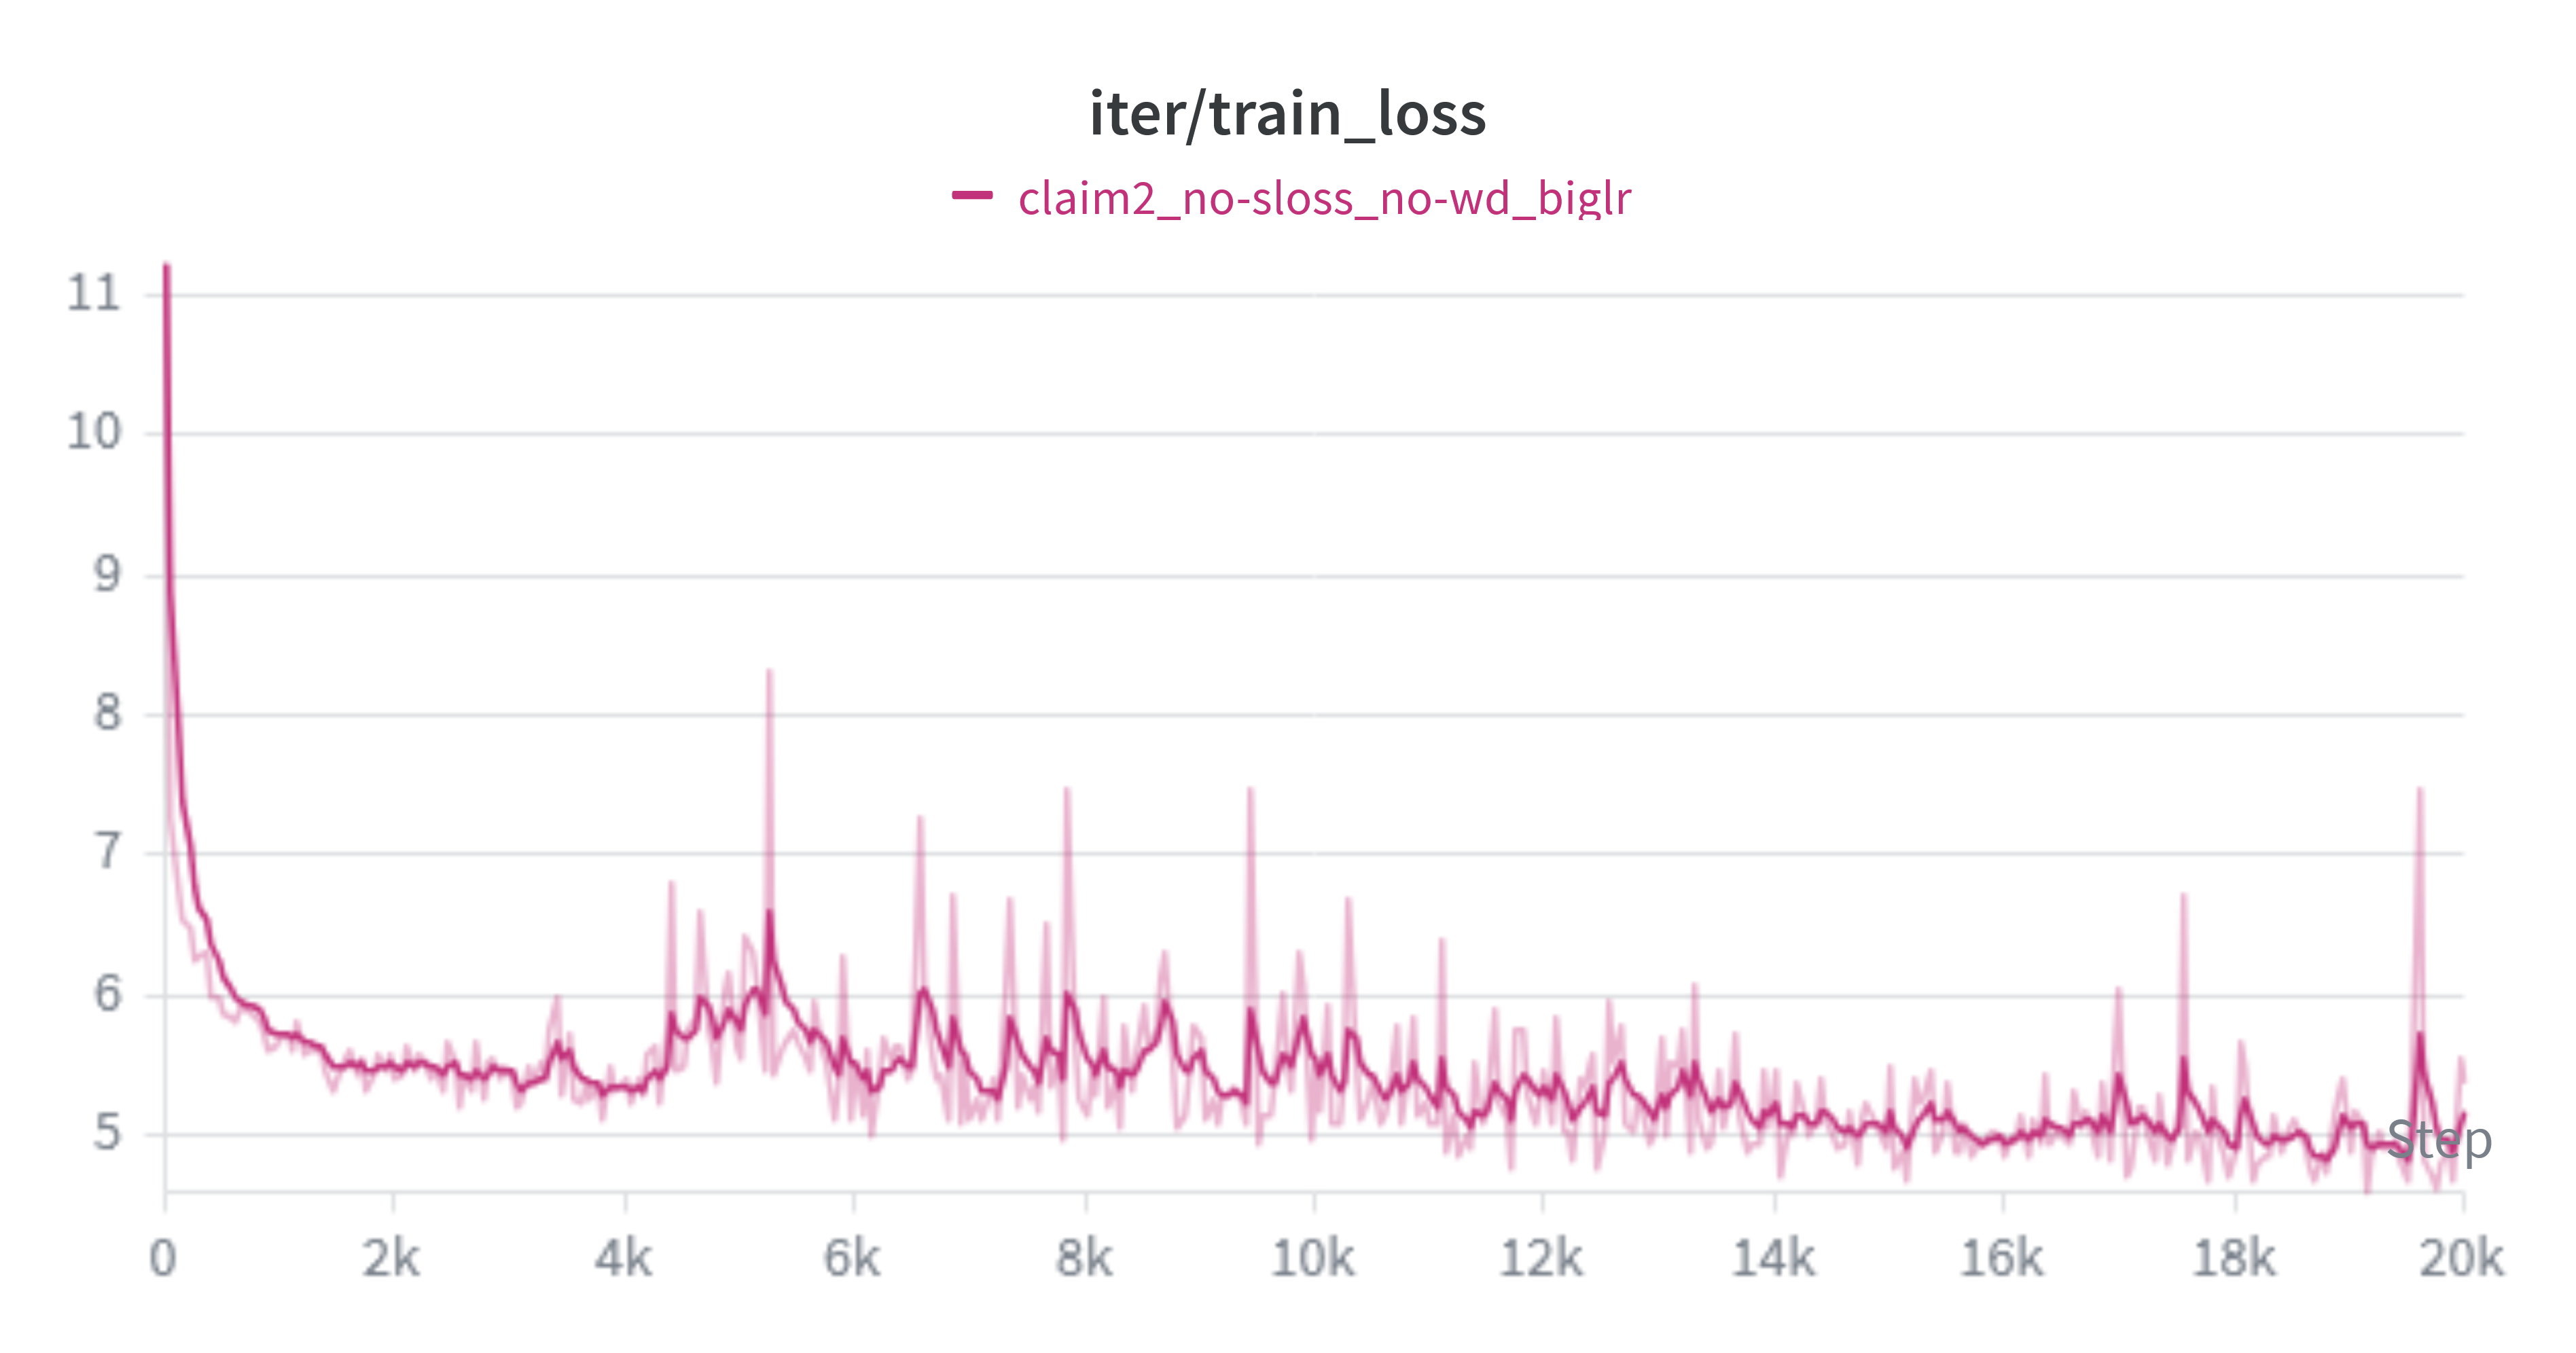
\includegraphics[width=\linewidth]{figures/C2_train_loss_mehstable.png}
        \caption{Moderately stable — train loss}
    \end{subfigure}
    \hfill
    \begin{subfigure}{0.48\textwidth}
        \centering
        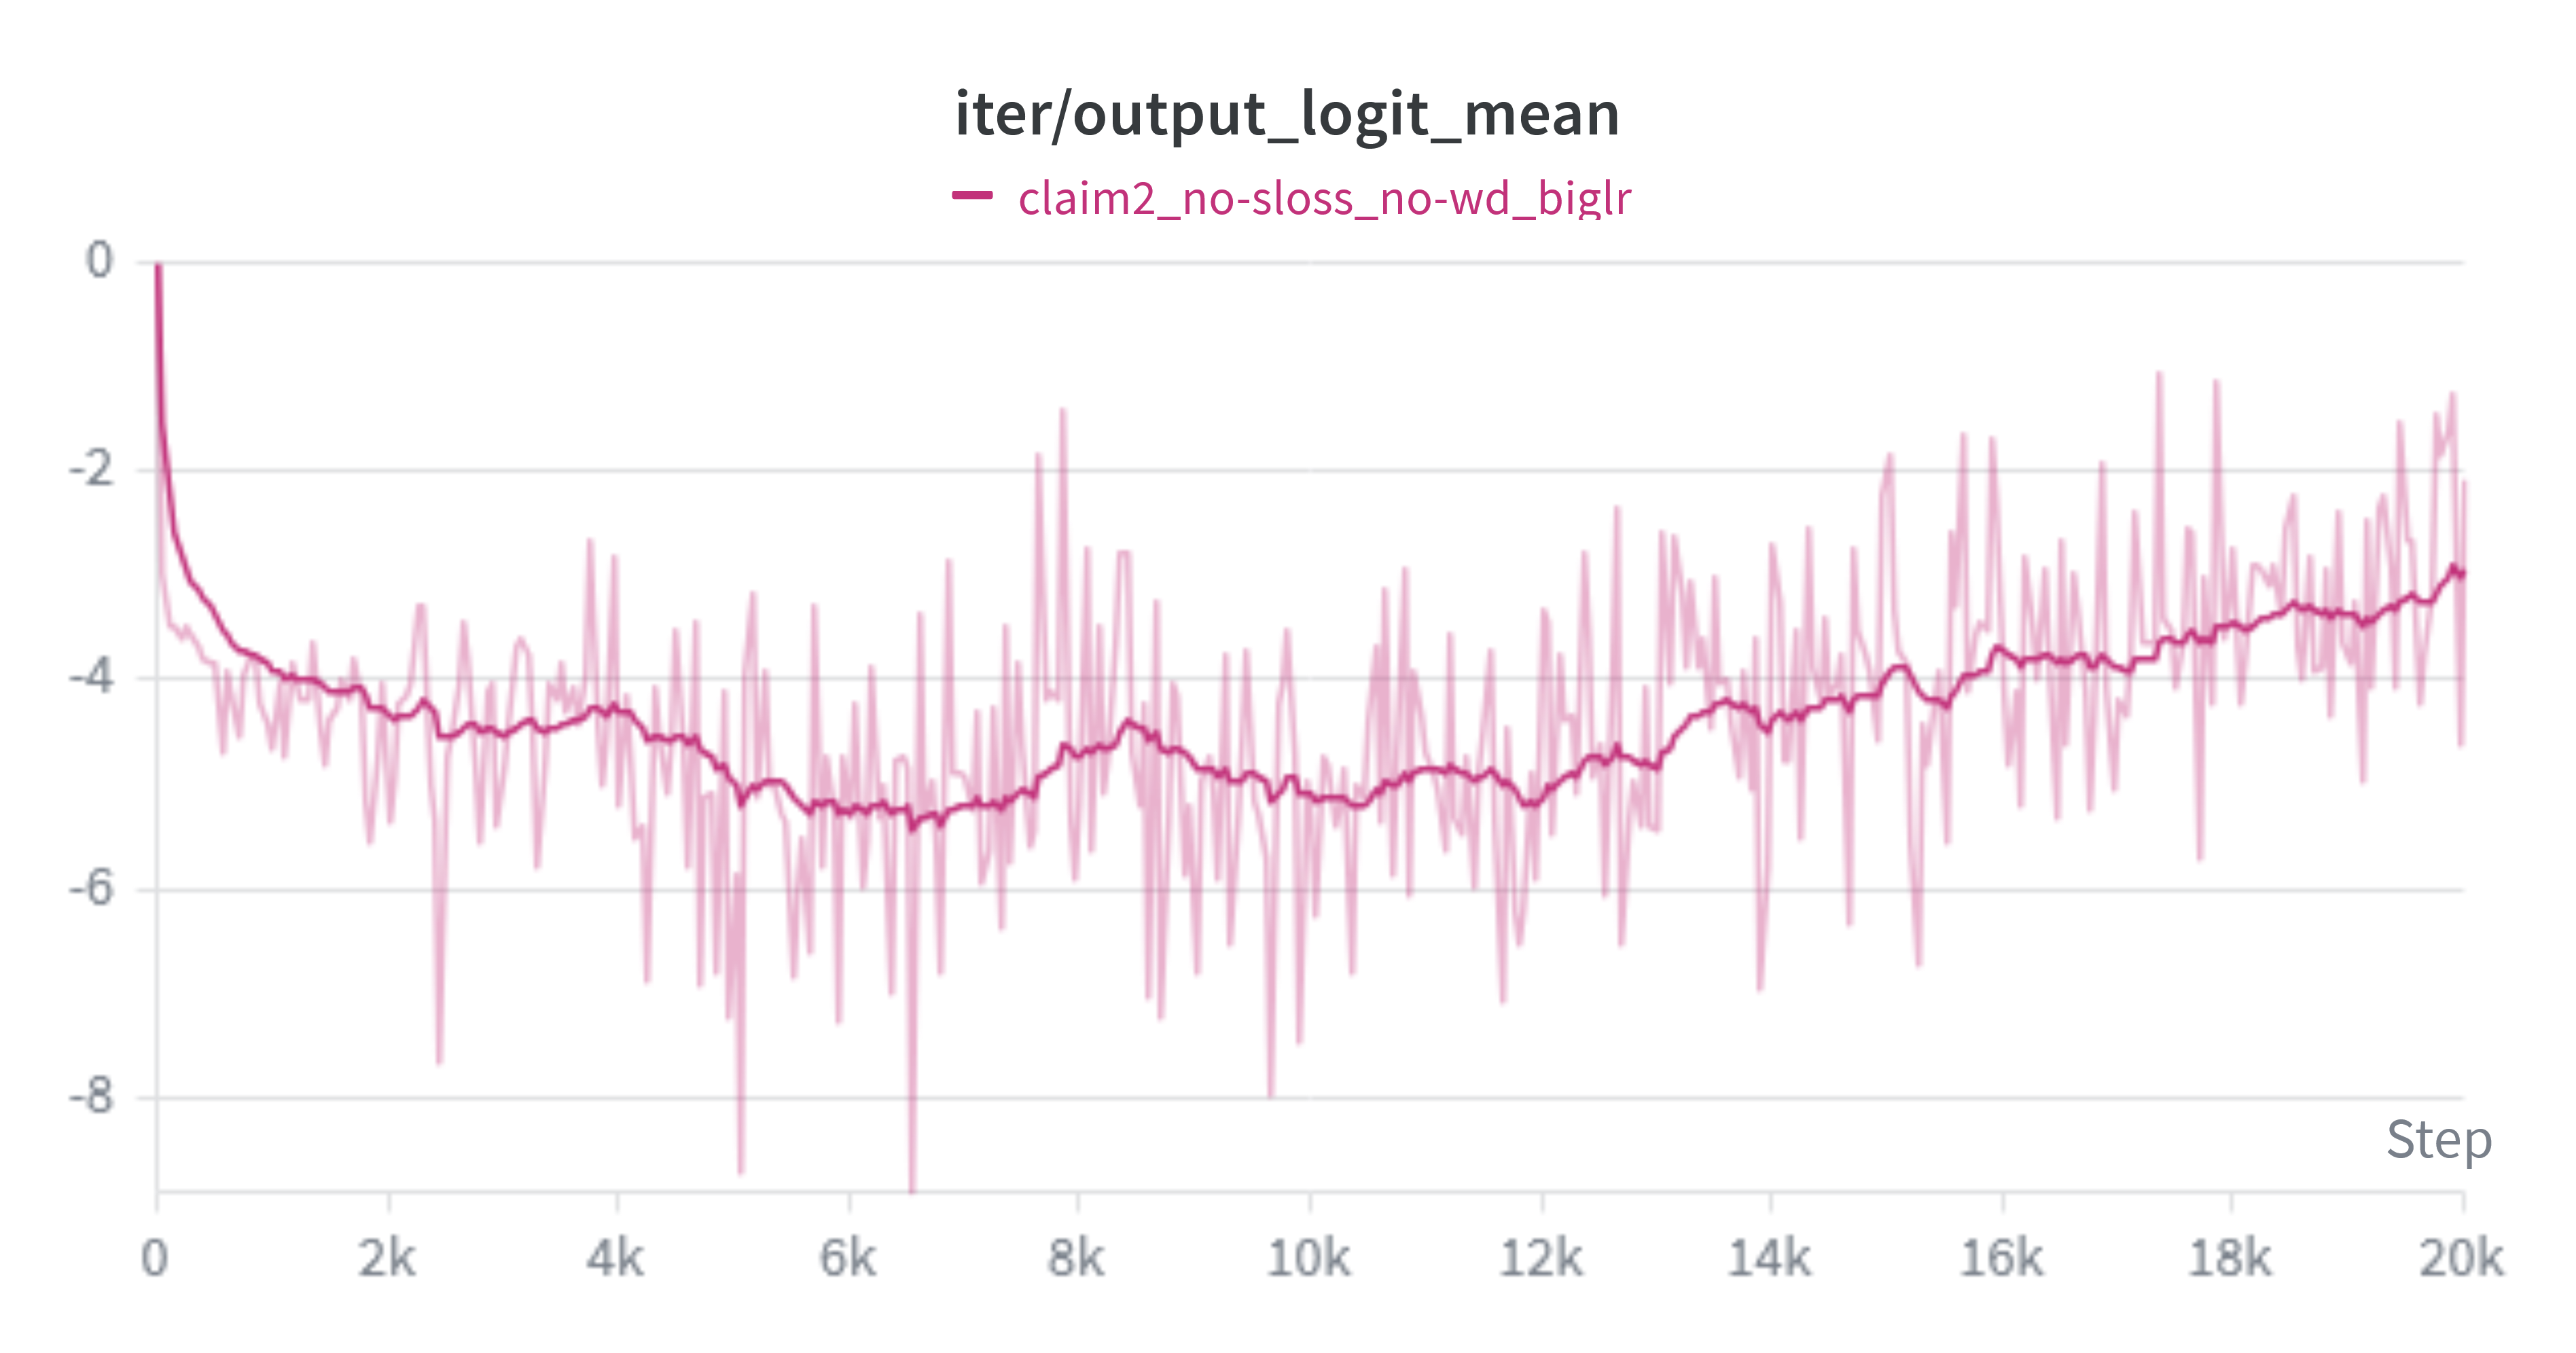
\includegraphics[width=\linewidth]{figures/C2_mean_meh_stable.png}
        \caption{Moderately stable — logit mean}
    \end{subfigure}

    \vspace{0.5em}

    % -------- Row 3: Unstable --------
    \begin{subfigure}{0.48\textwidth}
        \centering
        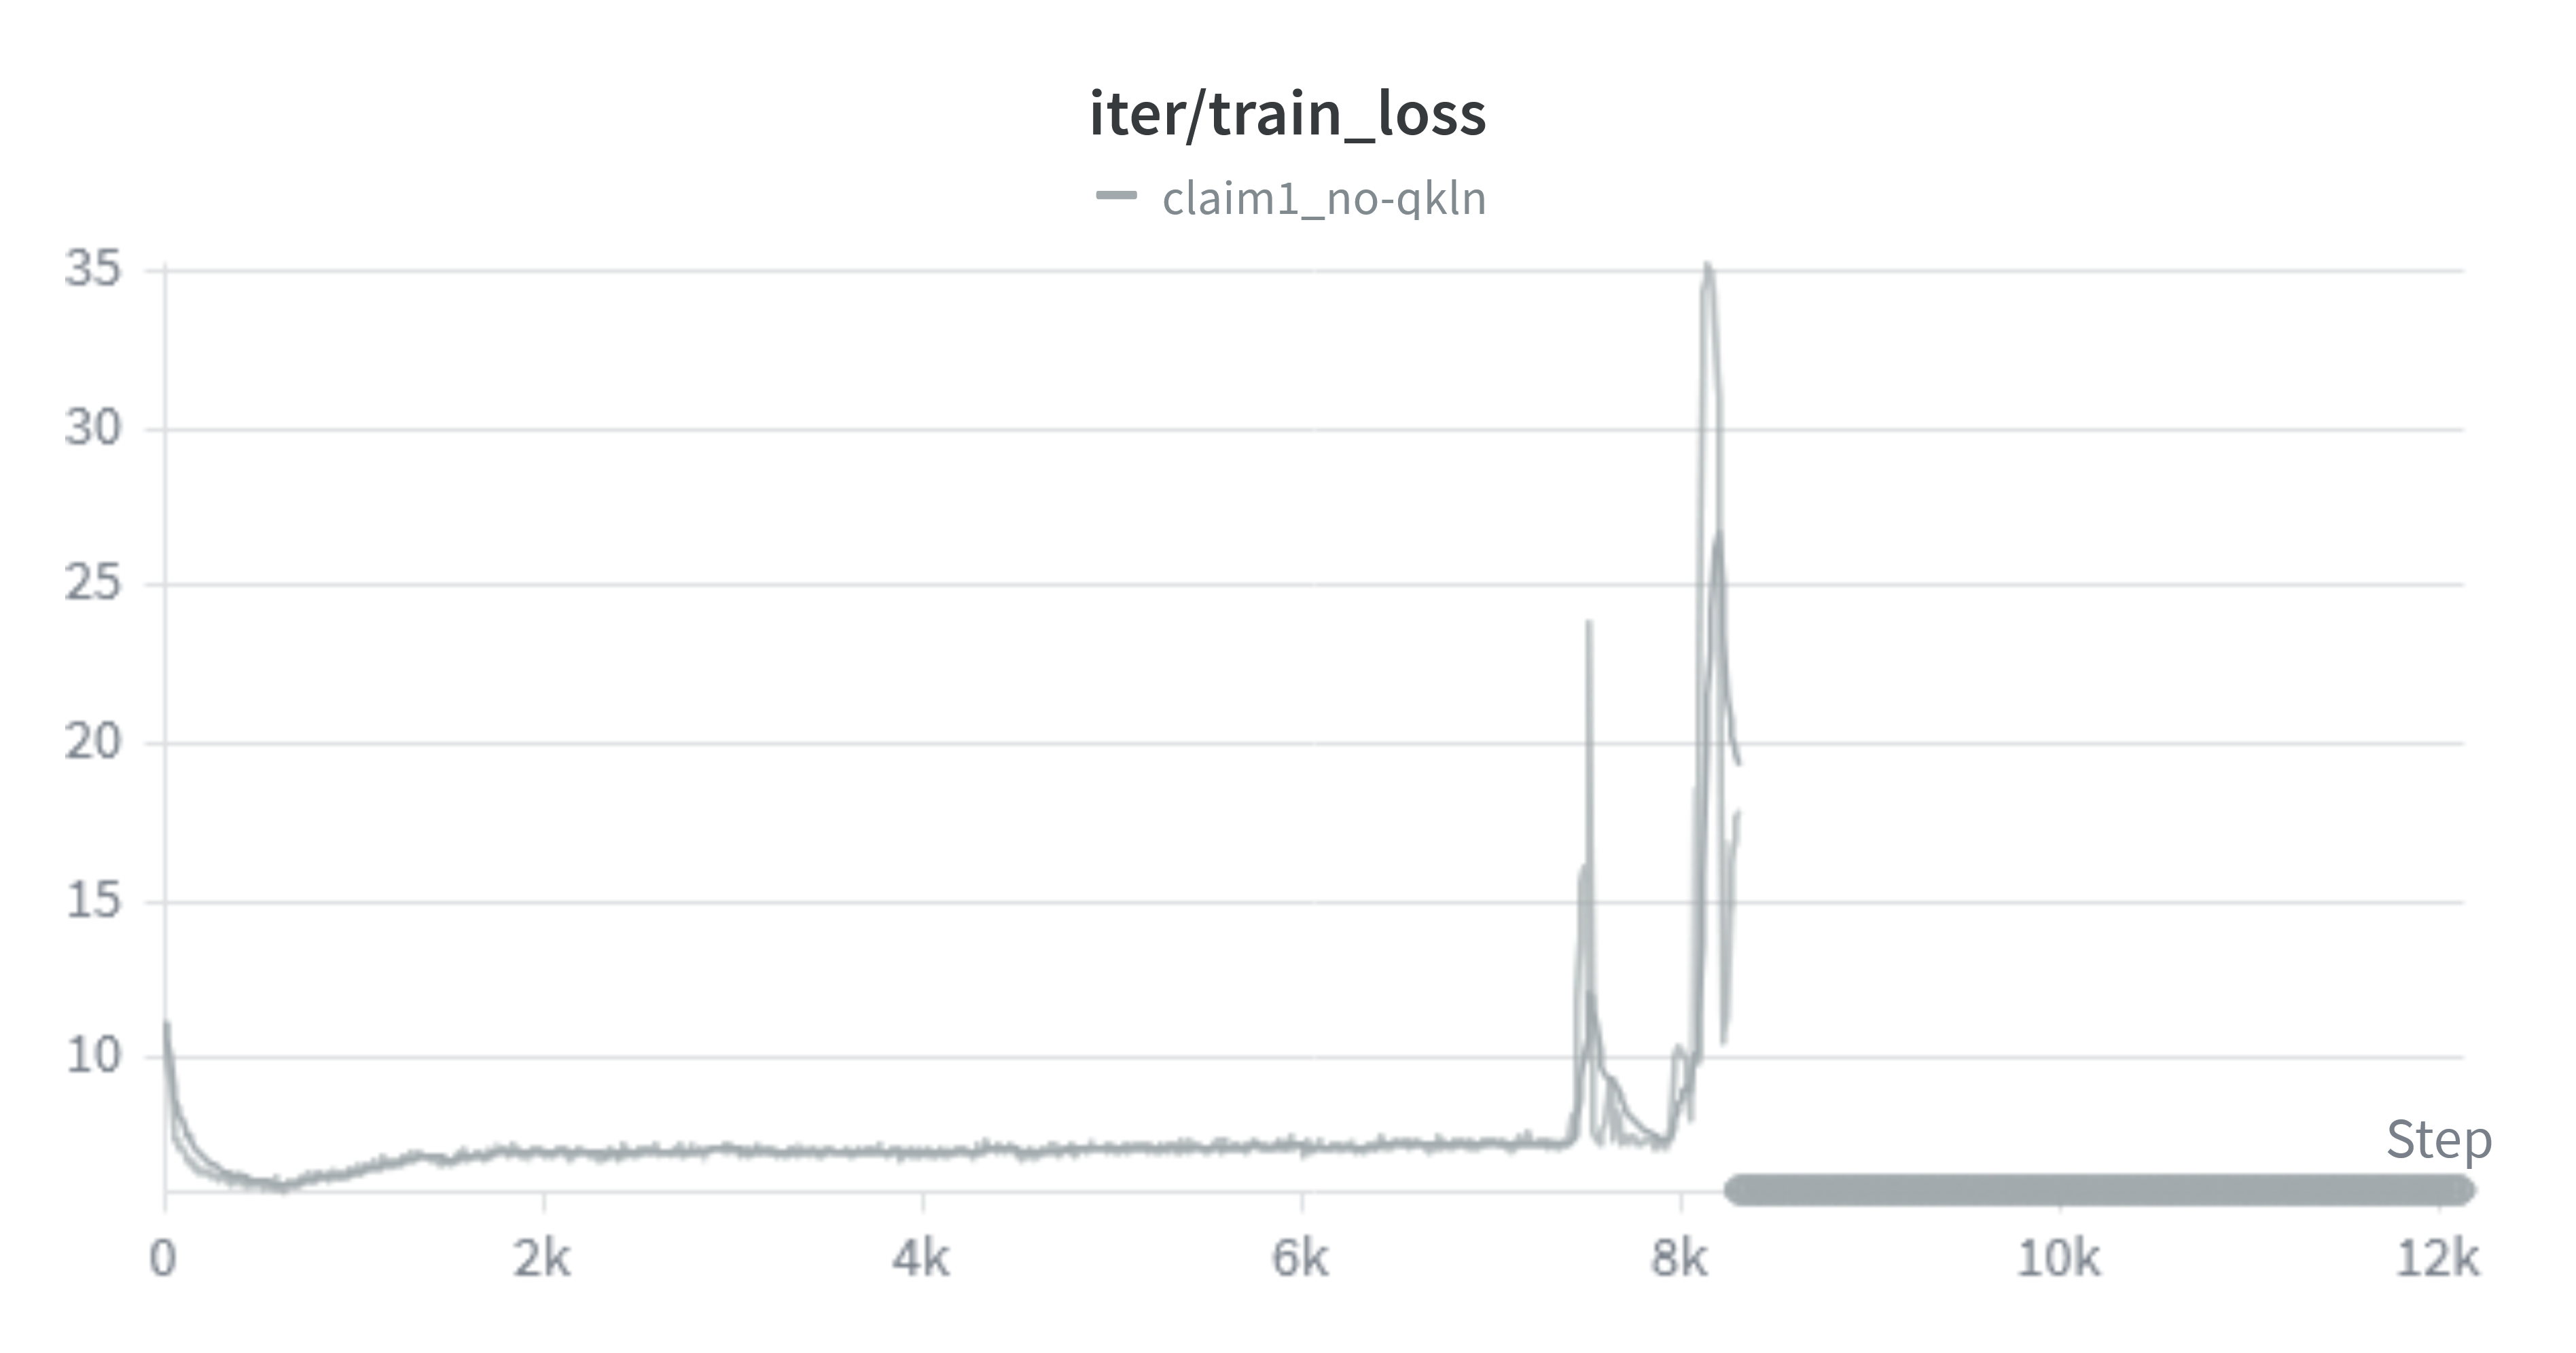
\includegraphics[width=\linewidth]{figures/C2_train_unstable.png}
        \caption{Unstable — train loss}
    \end{subfigure}
    \hfill
    \begin{subfigure}{0.48\textwidth}
        \centering
        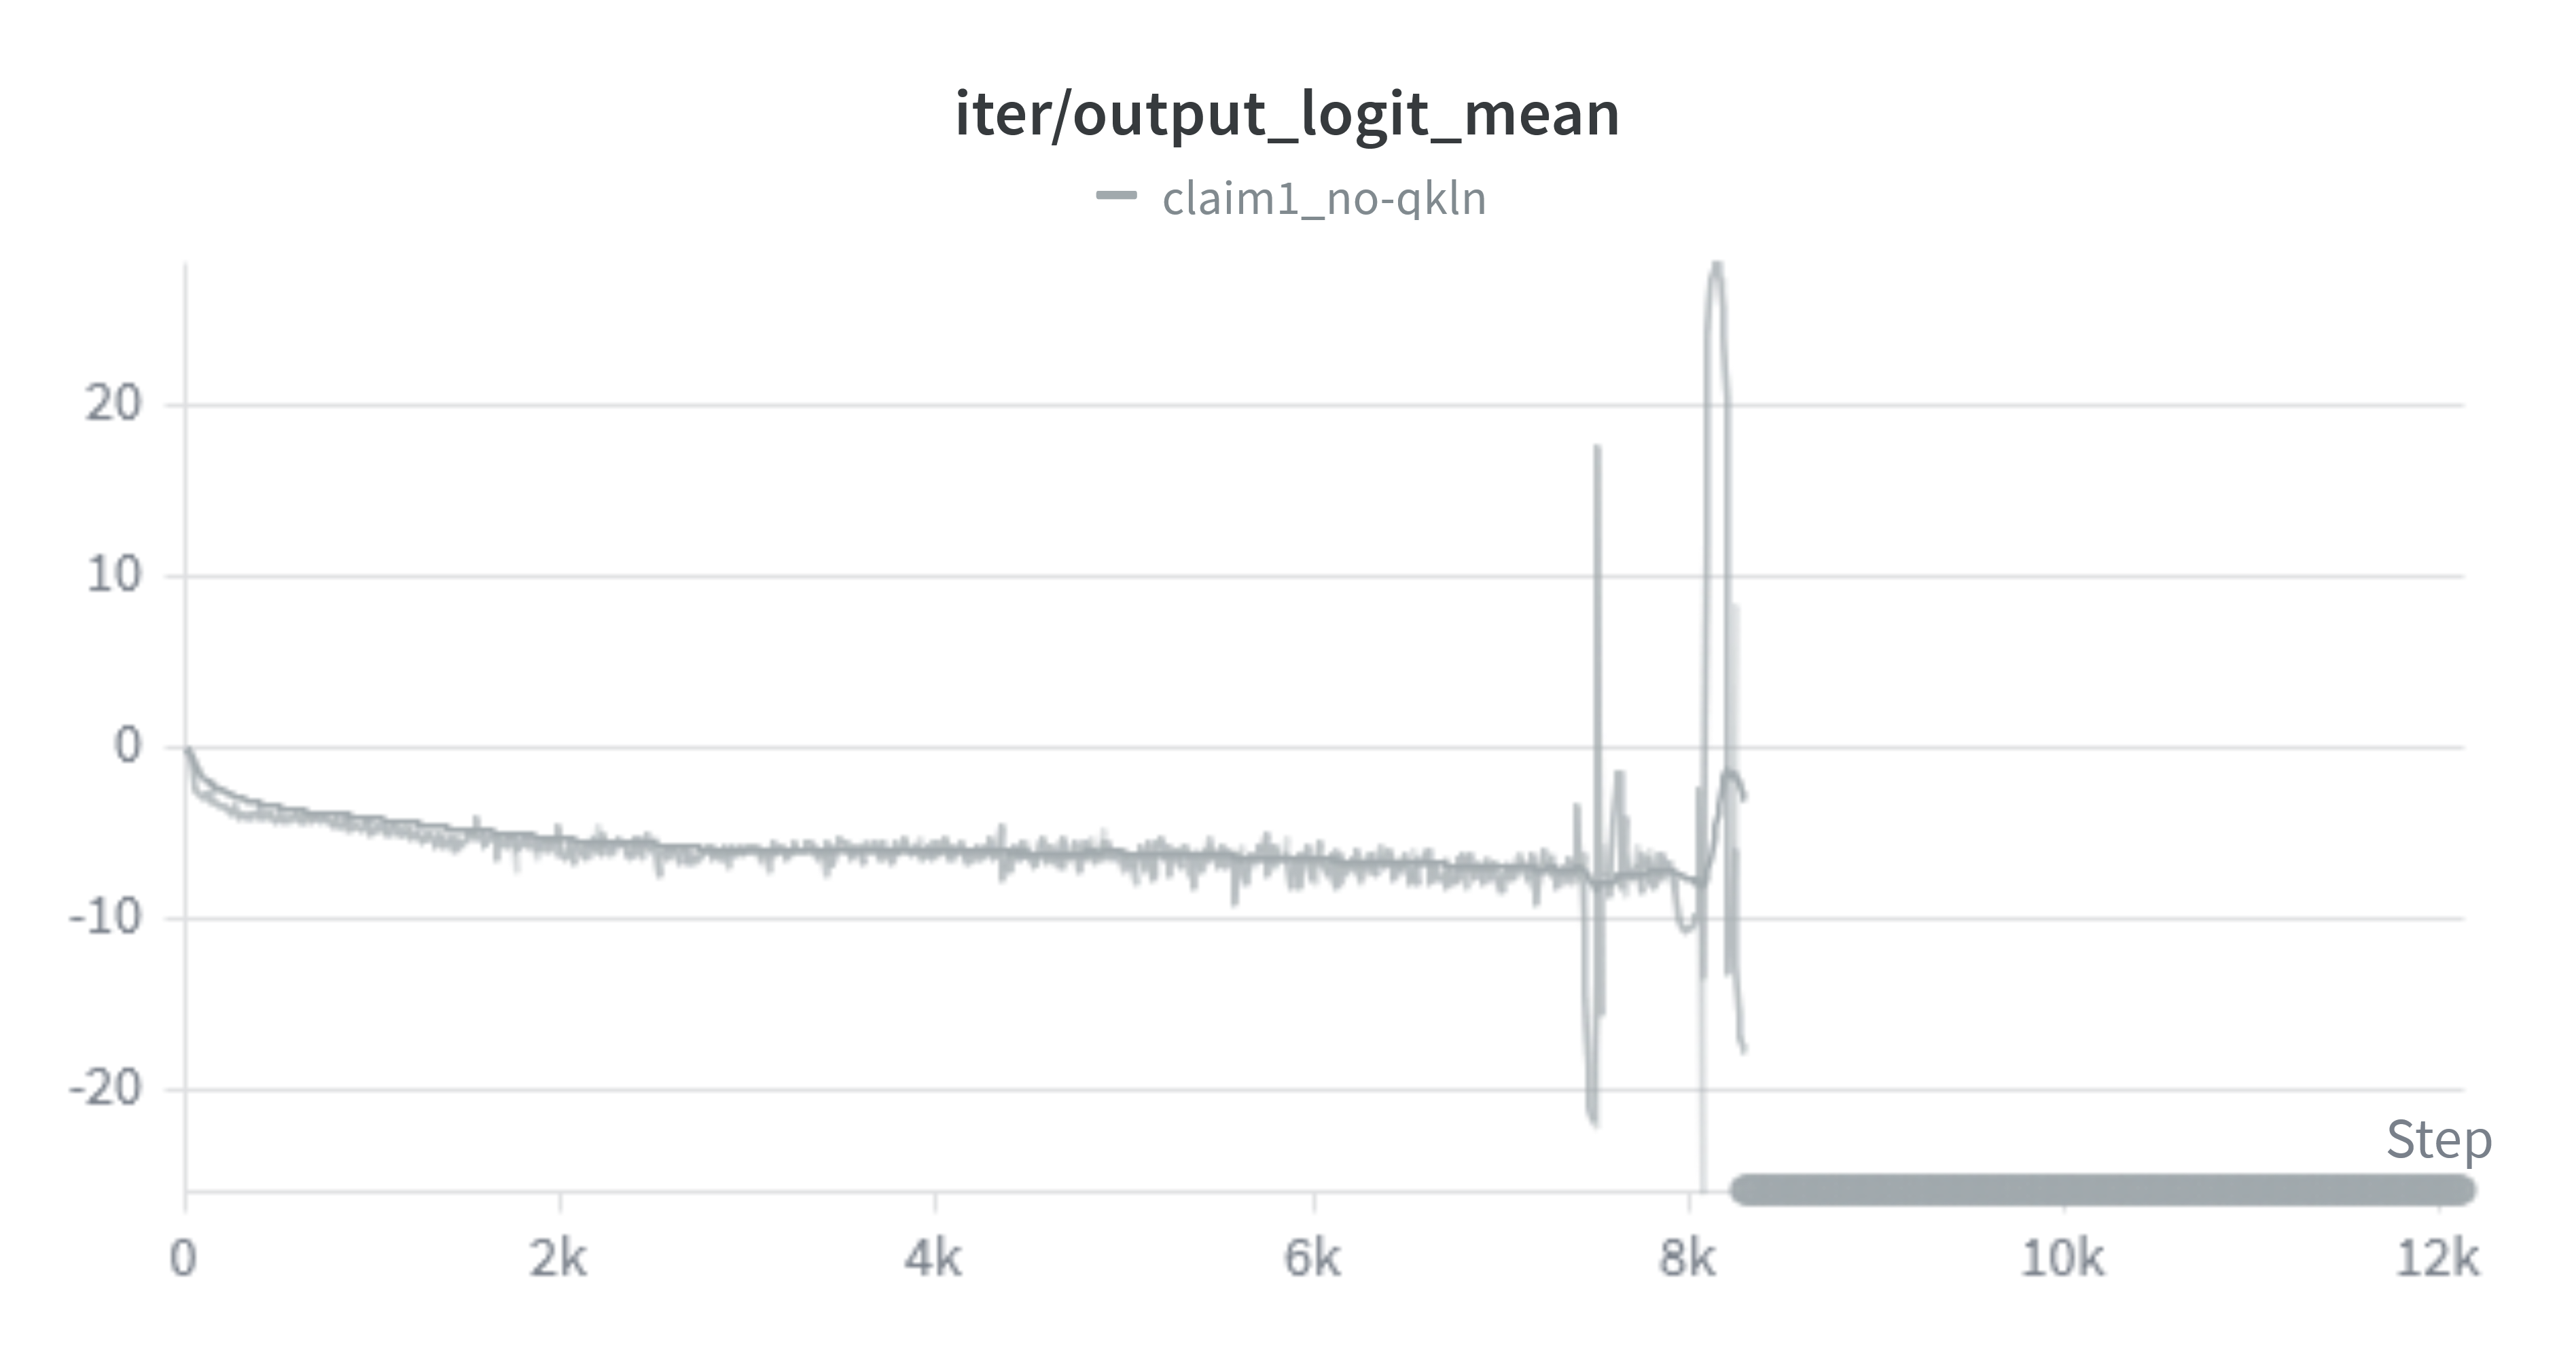
\includegraphics[width=\linewidth]{figures/C2_mean_unstable.png}
        \caption{Unstable — logit mean}
    \end{subfigure}

    \caption{Claim 2 experiments across three regimes. Top: stable training run(lr=0.1). Middle: moderately stable regime with mild fluctuations(lr linear warmup to 0.5). Bottom: unstable regime showing divergence. In three cases we did not observe a collapse to $-\infty$}
    \label{fig:claim2_grid}
\end{figure}
\paragraph{Takeaway.}
Our experiments therefore remain inconclusive for Claim~2.
They suggest that reproducing output-logit divergence may be more sensitive to
implementation details, model scale, or optimisation choices than suggested by
the simplified small-scale protocol alone.
